% Chapter: 02_llm_steganography
% Included from lectures/steganography/main.tex

\section{Steganography with LLMs}

\begin{frame}{PRF + LLM = Undetectable Steganography}
\begin{center}
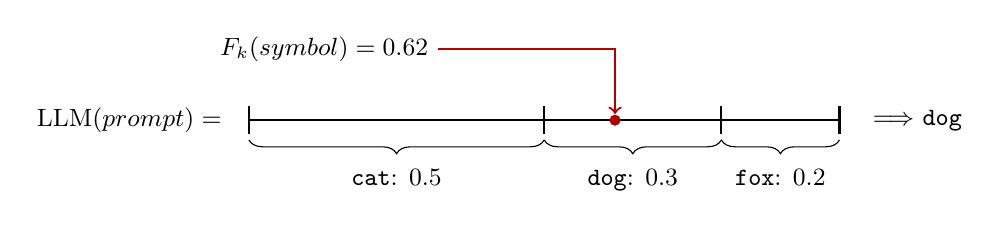
\begin{tikzpicture}[
  x=0.75cm,
  y=1cm,
  font=\small,
  tokenbrace/.style={decorate, decoration={brace, mirror, amplitude=5pt}},
]
  \draw[thick] (0, 0) -- (10, 0);
  \foreach \x in {0, 5, 8, 10}
    \draw[thick] (\x, -0.18) -- (\x, 0.18);

  \draw[tokenbrace] (0, -0.25) -- (5, -0.25) node[midway, below=7pt] {\texttt{cat}: $0.5$};
  \draw[tokenbrace] (5, -0.25) -- (8, -0.25) node[midway, below=7pt] {\texttt{dog}: $0.3$};
  \draw[tokenbrace] (8, -0.25) -- (10, -0.25) node[midway, below=7pt] {\texttt{fox}: $0.2$};

  \node[anchor=east] at (-0.3, 0) {$\mathrm{LLM}(\text{prompt}) =$};
  \node[anchor=east] (prf) at (3.2, 0.9) {$F_k(\text{symbol}) = 0.62$};
  \draw[thick, ->, red!70!black] (prf.east) -- (6.2, 0.9) -- (6.2, 0.08);
  \fill[red!70!black] (6.2, 0) circle (2pt);
  \node[anchor=west] at (10.4, 0) {$\Longrightarrow$ \texttt{dog}};
\end{tikzpicture}
\end{center}
\vspace{-0.3em}
\begin{itemize}
\item Normal sampling: draw a uniform $u \in [0, 1]$ and pick the token whose interval contains $u$
\item Steganography: replace $u$ by the output of a secret-keyed PRF that depends on the hidden symbol
\item The PRF output looks uniform, so the token distribution is unchanged
\item Any signal with entropy can be turned into a stego channel this way
\end{itemize}

\source{zamir2024}

\note{
\begin{itemize}
\item At every step the language model produces a probability distribution over the next token
\item Example: cat $0.5$, dog $0.3$, fox $0.2$
\item Normally the model samples a random number $u$ and chooses the token by cumulative probability intervals: cat if $u < 0.5$, dog if $0.5 \leq u < 0.8$, fox if $0.8 \leq u < 1$
\item The paper keeps this exact sampling procedure, but generates $u$ with a secret-keyed PRF instead of fresh randomness
\item The model still outputs cat, dog and fox with probabilities $0.5$, $0.3$, $0.2$
\item The hidden message is encoded by making the PRF input depend on the hidden symbol currently being transmitted
\item Sender and receiver share the PRF and the secret key $k$
\end{itemize}
}
\end{frame}

\begin{frame}{Sending and Decoding a Symbol}
\begin{columns}[T]
\begin{column}{0.47\textwidth}
\textbf{Sender}
\begin{itemize}
\item Wants to transmit a symbol $\sigma \in \{\texttt{0}, \texttt{1}, \leftarrow\}$
\item Samples with randomness
$$F_k(r, i, \sigma)$$
\item $k$: secret key, $i$: token position, $r$: prefix of this response
\item Pushes the same symbol for several consecutive tokens
\end{itemize}
\end{column}
\begin{column}{0.47\textwidth}
\textbf{Receiver}
\begin{itemize}
\item Knows $k$, sees the tokens
\item Keeps a score for every candidate symbol $\texttt{0}, \texttt{1}, \leftarrow$
\item The score of the correct symbol tends to grow faster
\item Once a score crosses a threshold $t$: record the symbol, reset the scores
\end{itemize}
\end{column}
\end{columns}

\source{zamir2024}

\note{
\begin{itemize}
\item To transmit a code symbol the generator uses randomness $F_k(r, i, \sigma)$
\item $k$ is the secret key, $i$ is the token position, $r$ is a response-specific random prefix
\item For several consecutive tokens the generator samples using the PRF stream of the current symbol
\item The visible text still follows the normal LLM distribution
\item The decoder knows $k$, so for the observed tokens it computes scores for each candidate symbol
\item The correct symbol's score tends to grow faster
\item Once one score crosses a threshold, the decoder records that symbol and resets the scores
\item Then the sender moves on to the next symbol
\end{itemize}
}
\end{frame}

\begin{frame}{Error Correction and Capacity}
\begin{itemize}
\item \textbf{LLM and prompt known}: the receiver can decode perfectly
\item \textbf{Only the tokenizer known}: the receiver decodes probabilistically and sometimes accepts a wrong symbol
\item The payload is encoded with an error-correcting code over $\{\texttt{0}, \texttt{1}, \leftarrow\}$
\item $\leftarrow$ is a \textbf{backspace}: it repairs an earlier decoding error
\item With an error rate below $0.5$ there is net progress towards the correct message
\end{itemize}
\vspace{0.5em}
\begin{itemize}
\item \textbf{Capacity}: longer, higher-entropy responses carry more payload
\item \textbf{Reuse}: each response starts with a natural high-entropy prefix $r$ that enters all later PRF inputs, so every response gets fresh keyed randomness
\end{itemize}

\source{zamir2024}

\note{
\begin{itemize}
\item Scenario 1: LLM and prompt are known, the receiver can decode perfectly
\item Scenario 2: only the tokenizer is known, the receiver can still decode probabilistically with error correction
\item Because the decoder can occasionally pick the wrong symbol, the hidden payload is first encoded with a dynamic error-correcting code
\item If a wrong symbol got accepted, the sender sends a backspace symbol
\item As long as the error rate is below $0.5$, the process has net progress towards correct symbols
\item The response contains as many hidden symbols as its length and entropy allow
\item For full security across many queries the model first generates a natural high-entropy prefix $r$, which is included in later PRF inputs
\end{itemize}
}
\end{frame}

\begin{frame}{From Steganography to Watermarking}
A watermark is steganography with a \textbf{one-bit payload}: ``this text came from our model''.
\vspace{0.5em}
\begin{itemize}
\item Same construction: the sampler's randomness comes from a keyed pseudorandom function of the key and the preceding tokens
\item Different goal: robust detection, and the adversary wants to \emph{remove} the mark
\end{itemize}
\vspace{0.5em}
\begin{description}
\item[2022] Scott Aaronson and Hendrik Kirchner propose the Gumbel scheme at OpenAI
\item[2024] SynthID-Text by Google DeepMind, based on tournament sampling
\item[2026] Claude's text watermark, a version of the SynthID-Text approach, announced in August for the EU AI Act transparency rules
\end{description}

\source{aaronson2022,dathathri2024}

\note{
\begin{itemize}
\item The steganography paper extends earlier work by Christ, Gunn and Zamir on undetectable watermarks
\item A watermark only says: this came from the model, there is no message to decode
\item Anthropic describes Claude's watermark as a version of the SynthID-Text approach, in a family of approaches that goes back to Aaronson's 2022 proposal
\item The method is public, the key and the exact parameters are not
\item Nothing is added to the text, there are no hidden characters
\item Detection works badly on short texts and on passages with few free choices, such as code
\item Light editing does not remove it, a complete rewrite does
\end{itemize}
}
\end{frame}

\begin{frame}{The Gumbel Watermark}
\begin{columns}[T]
\begin{column}{0.47\textwidth}
\textbf{Generation}
\begin{itemize}
\item Model gives probabilities $p_v$
\item One pseudorandom number per token $v$:
$$r = F_k(\text{previous tokens}) \in [0, 1]^{|V|}$$
\item Output
$$x = \arg\max_v \; r_v^{1/p_v}$$
\item Token $v$ wins with probability exactly $p_v$
\end{itemize}
\end{column}
\begin{column}{0.47\textwidth}
\textbf{Detection}
\begin{itemize}
\item Needs the key and the text, not the model
\item Recompute $r$ for every observed token $x_i$
$$S = \sum_{i=1}^{n} -\ln\left(1 - r_{x_i}\right)$$
\item No watermark: $S \sim \mathrm{Gamma}(n, 1)$, mean $n$
\item Watermark: $S$ is larger, the gap grows with the entropy of the text
\end{itemize}
\end{column}
\end{columns}

\source{aaronson2023}

\note{
\begin{itemize}
\item This is the scheme you will implement in the exercise
\item The key and the previous few tokens seed the pseudorandom numbers
\item The argmax rule is the Gumbel-max trick: over random $r$ token $v$ wins with probability exactly $p_v$, so the output distribution is unchanged
\item But the chosen token tends to have $r_v$ close to $1$
\item Detection: without a watermark the $r$ values of the observed tokens are uniform, so each term is exponential with mean $1$
\item The sum of $n$ such terms follows a Gamma distribution with shape $n$, which gives a p-value
\item Low-entropy text leaves the model few choices, so it carries little watermark
\end{itemize}
}
\end{frame}

\begin{frame}{}
\centering
\Large \href{https://colab.research.google.com/github/wusche1/Iliad_steganography_and_backdoors/blob/main/exercises/watermarking/notebook.ipynb}{\textbf{Exercise 1: Watermarking}} \\[1em]
\normalsize 30 minutes \\[1em]
\qrcode[height=3cm]{https://colab.research.google.com/github/wusche1/Iliad_steganography_and_backdoors/blob/main/exercises/watermarking/notebook.ipynb}

\note{
\begin{itemize}
\item Implement the pseudorandom function, the Gumbel sampling rule and the detector
\item Then run the experiments on text length, entropy and editing
\item Bonus: hide a message instead of a single bit, which turns the watermark into the steganography scheme from the talk
\end{itemize}
}
\end{frame}
